% f2015hbl_q14_circle.tex — 2015 年高考数学·湖北卷·理科 第 14 题（圆与单位圆）
%
% 【来源】`.work/phase3-b21/source/2015湖北理.pdf`（SHA-256
%   66e6822009bdfd8f9a5a4adf4dd3f7564fc74d8fa09906c271dc6c6a5b31a66f），
%   第 1 页（合订本页 951）；内容对象 5/7/9/…/19。逐路径实测见
%   `.work/phase3-b21/figure-inventory.md`。
%
% 【坐标口径】源 PDF 用户空间（原点左下、y 向上）。本图本地坐标
%   (x, y) = (x_page − 523.384, y_page − 56.892)，1 单位 = 1 TeX pt。
%   路径坐标逐点照录内容流（含三次贝塞尔控制点）。
%
% 元素计数：9 条路径（x/y 轴＋箭头、单位圆 O、圆 C、三角形 MBN 三边）＋10 个标签（含圆心点）
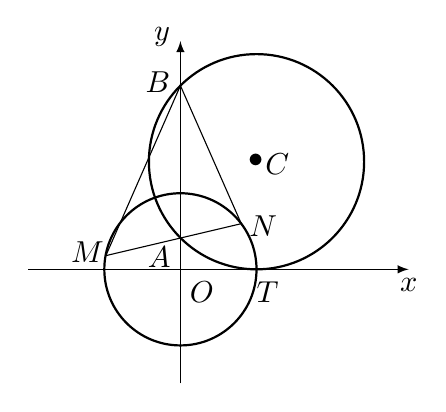
\begin{tikzpicture}[x=1pt, y=1pt,
    every node/.style={inner sep=0pt, font=\fontsize{10.5pt}{12.6pt}\selectfont}]
  \draw[line width=0.398pt] (0.0001,41.2450)   -- (133.8961,41.2450);
  \fill[line width=1.0pt] (137.4823,41.2450)   .. controls (136.4193,41.4440) and (134.6923,42.0420) .. (133.4973,42.7390)   -- (133.4973,39.7510)   .. controls (134.6923,40.4480) and (136.4193,41.0460) .. (137.4823,41.2450);
  \draw[line width=0.398pt] (54.9930,0.0004)   -- (54.9930,120.1474);
  \fill[line width=1.0pt] (54.9930,123.7343)   .. controls (54.7940,122.6713) and (54.1960,120.9443) .. (53.4990,119.7493)   -- (56.4870,119.7493)   .. controls (55.7900,120.9443) and (55.1920,122.6713) .. (54.9930,123.7343);
  \draw[line width=0.797pt] (82.4894,41.2450)   .. controls (82.4894,56.4310) and (70.1794,68.7410) .. (54.9934,68.7410)   .. controls (39.8074,68.7410) and (27.4964,56.4310) .. (27.4964,41.2450)   .. controls (27.4964,26.0590) and (39.8074,13.7490) .. (54.9934,13.7490)   .. controls (70.1794,13.7490) and (82.4894,26.0590) .. (82.4894,41.2450)   -- cycle;
  \draw[line width=0.398pt] (54.9930,107.6273)   -- (28.0470,46.1943);
  \draw[line width=0.398pt] (54.9930,107.6273)   -- (76.9900,57.7433);
  \draw[line width=0.398pt] (28.0466,46.1941)   -- (76.9906,57.7431);
  \draw[line width=0.797pt] (121.3753,80.1309)   .. controls (121.3753,101.6069) and (103.9653,119.0169) .. (82.4893,119.0169)   .. controls (61.0133,119.0169) and (43.6033,101.6069) .. (43.6033,80.1309)   .. controls (43.6033,58.6549) and (61.0133,41.2449) .. (82.4893,41.2449)   .. controls (103.9653,41.2449) and (121.3753,58.6549) .. (121.3753,80.1309)   -- cycle;

  \node[anchor=center] at (48.366,125.148) {$y$};  % 源中心 (571.75,182.04)
  \node[anchor=center] at (46.816,109.048) {$B$};  % 源中心 (570.20,165.94)
  \node[anchor=center] at (82.466,80.598) {$\bullet$};  % 源中心 (605.85,137.49)
  \node[anchor=center] at (89.966,79.148) {$C$};  % 源中心 (613.35,136.04)
  \node[anchor=center] at (84.916,56.748) {$N$};  % 源中心 (608.30,113.64)
  \node[anchor=center] at (21.416,47.548) {$M$};  % 源中心 (544.80,104.44)
  \node[anchor=center] at (47.366,45.748) {$A$};  % 源中心 (570.75,102.64)
  \node[anchor=center] at (62.716,32.998) {$O$};  % 源中心 (586.10,89.89)
  \node[anchor=center] at (86.466,32.998) {$T$};  % 源中心 (609.85,89.89)
  \node[anchor=center] at (137.516,35.648) {$x$};  % 源中心 (660.90,92.54)

\end{tikzpicture}
%
% 【自验结果】
%   探针：latexmk -pdfxe（待跑）。
